\subsection{Model Diagnostics}
\label{sec:algeval}

Machine learning algorithms are heavily dependent on the inputs and parameters
given to them, such as training set sizes, regularization, learning rates, etc.
From the results shown in Section \ref{sec:statmodel}, it is clear there is
room for improvement.  The diagnostic plots show the errors of the predicted
burnup values to the actual burnup values with respect to some variable on the
\textit{x}-axis.  As previously introduced in Section \ref{sec:optvalid}, the
errors are compared to the training error to understand the generalization
strength with respect to training set size (learning curves) and the algorithm
parameters governing model complexity (validation curves). 

In addition to machine learning best practices, another layer of comparison is
added here.  Because it is difficult to ensure consistently representative
testing data, the accuracy of a learned model should not depend on only one
testing set.  The learned model's accuracy is better estimated by using a
validation set, or even better, \textit{k}-fold cross-validation, introduced in
Section \ref{sec:selectass} This work includes both the testing error (using
the testing set described in Section \ref{sec:training}) and cross-validation
error. The predetermined testing set will allow for comparison against the
previous work it was obtained from, but it is assumed that cross-validation
will provide a better indication of model performance.

\begin{figure}[!htb]
    \centering
    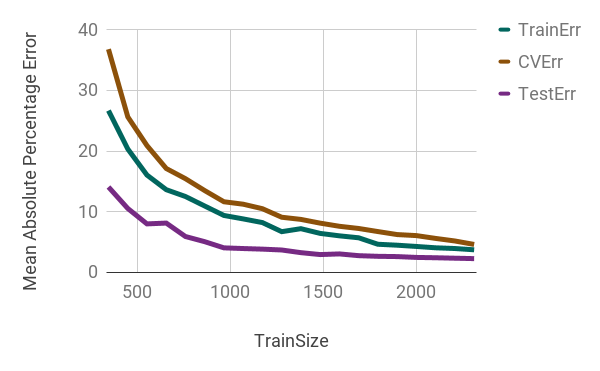
\includegraphics[width=\linewidth]{./chapters/demo_method/lc1.png}
    \caption{Learning curve for burnup prediction, $\gamma = 0.001$}
    \label{fig:lc1}
\end{figure}

The learning curves are obtained as follows, shown in Figure \ref{fig:lc1}.
For a given (randomly chosen) training set size between 15 and 100\% of the
total data set, training and prediction rounds were performed for each. The
testing error scenario performs this \textit{k} times and averages those
results.  This is equivalent to the \textit{k} in \textit{k}-fold
cross-validation to provide some semblance of equivalent statistics.  The
cross-validation error scenario has no need for averaging because it is
performed automatically. In both cases, the learning curves do not provide a
clear picture of over- or undertraining upon first glance.

\begin{figure}[!htb]
    \centering
    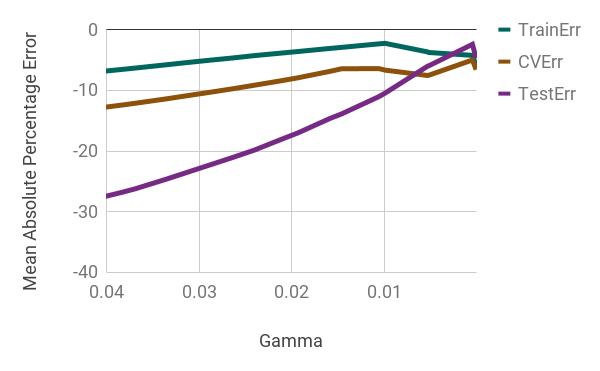
\includegraphics[width=\linewidth]{./chapters/demo_method/vc1.png}
    \caption{Validation curve for burnup prediction, $TrainSize = 2313$}
    \label{fig:vc1}
\end{figure}

The validation curves are obtained as follows, shown in Figure \ref{fig:vc1}.
The $\gamma$ parameter in \gls{SVR}, which influences model complexity, was
varied from $10^{-4}$ to $10^{-1}$. Training and prediction rounds were
performed for different $\gamma$ values in this range.  Again, the testing and
cross-validation errors are both used as described above. As with Figure
\ref{fig:lc1}, determining the robustness to over- or undertraining is
difficult here although there is possibly a minimum at $\gamma = 0.001$.

Although there is no example behavior of Figure \ref{fig:lc1}'s peculiar
learning curve in Figure \ref{fig:learning}, the curve mimics the squared bias
curve from Figure \ref{fig:bvtradeoff}. This indicates that the bias in the
model is much higher than the variance.  Next, the testing error is lower than
the training error; this should never be the case, and indicates an issue with
the systematically chosen testing set.  While the cross-validation error is
correctly higher than the training error, it follows along in parallel,
producing no information on model fitness other than confirming a very high
bias.  It is presumed this is not the fault of the algorithms, but the training
set itself.  It is likely covering too small of a range of the simulation
space.

Additionally, Figure \ref{fig:vc1}'s validation curve shows the testing error
dropping below the training error for extremely small $\gamma$, around where a
minimum might be.  Since the model suffers from high bias, no amount of model
complexity can be optimized. 

%%%%%%%%%%%%%%%%%%%%%%%%%%%%%%%%%%%%%%%%%%%%%%%%%%%%%%%%%%%%%%%%%%%%%%%%%%%%%
%%%%%%%%%%%%%%%%%%%%%%%%%%%%%%%%%%%%%%%%%%%%%%%%%%%%%%%%%%%%%%%%%%%%%%%%%%%%%
The resolution to the underfitting is discussed
To obtain reliable models, one must both choose or create a training set
carefully and study the impact of various algorithm parameters on the error.
Many algorithms are developed on an assumption that the training set will be
independent and identially distributed (i.i.d.). This is important so that the
model does not overvalue or overfit a certain area in the training space. The
testing error can therefore be tabulated with respect to training set size,
number of features, or algorithm parameters (regularization terms, etc). The
results are broadly known as diagnostic plots. 

The next step is to provide a larger, more diverse training set to the
algorithms so they could predict better when faced with new instances.  Dayman
training/test set -> sfcompo-like sims and testing set
%%%%%%%%%%%%%%%%%%%%%%%%%%%%%%%%%%%%%%%%%%%%%%%%%%%%%%%%%%%%%%%%%%%%%%%%%%%%%
%%%%%%%%%%%%%%%%%%%%%%%%%%%%%%%%%%%%%%%%%%%%%%%%%%%%%%%%%%%%%%%%%%%%%%%%%%%%%

Lastly, it must be noted that the errors here are all measured in \gls{MAPE}.
While this is more intuitively convenient, it requires ensuring that no true
values are $0$. Thus, \gls{RMSE} is the preferred error measurement used in
the community and will be used in all future work.

%%%%%%%%%%%%%%%%%%%%%%%%%%%%%%%%%%%%%%%%%%%%%%%%%%%%%%%%%%%%%%%%%%%%%%%%%%%%%
%%%%%%%%%%%%%%%%%%%%%%%%%%%%%%%%%%%%%%%%%%%%%%%%%%%%%%%%%%%%%%%%%%%%%%%%%%%%%
\subsection{Model Comparison}
\label{sec:algcompare}
%%%%%%%%%%%%%%%%%%%%%%%%%%%%%%%%%%%%%%%%%%%%%%%%%%%%%%%%%%%%%%%%%%%%%%%%%%%%%
%%%%%%%%%%%%%%%%%%%%%%%%%%%%%%%%%%%%%%%%%%%%%%%%%%%%%%%%%%%%%%%%%%%%%%%%%%%%%

Regression Training Error: Confidence intervals on predictions to understand
true error versus sample error Test set must be > 30 instances, Can easily
calculate N\% confidence interval.

Options for comparison of algorithms: inverse bayesian stuff, comparing
classification of 2 classes on same ROC plot with multiple ML systems, Scatter
plots, Pairwise t-tests.
\todo{Discuss understanding confidence intervals in predictions.}

Alg Compare: inverse prob theory
In addition to evaluating a single learned model, it may be beneficial to
compare models. As discussed in \todo{the algorithm comparison section}, there
are three methods that will be used: comparison of \gls{ROC} curves, scatter
plots, and pairwise \textit{t}-tests.

